\section{Triangular matrices and invertible corners}
\label{corner:sec:corners}

Continue under the no-finite-win assumption and fix the symmetric price
of \cref{thm:prices}. Our goal is contraction to an invertible submatrix.

\begin{theorem}[Invertible corners]
\label{thm:corner}
If an invertible matrix $K$ has an invertible square submatrix $M$,
then $p(M)\le p(K)$.
\end{theorem}

Independent row and column permutations move $M$ to a corner without
changing the price of $K$. To compare their prices, we will run the
resulting block matrix along many tensor axes and for many time steps.
The other coordinates persist as state between successive steps. Their
initial values affect the output, so the main task is to remove that
contribution at a cost small compared with the number of calls.

We first obtain price bounds for rectangular shears and scalar
convolutions. We then prove that a block triangular matrix costs at
least the sum of its diagonal blocks. These tools allow us to correct
the initial state in a long cascade and isolate the repeated tensor
powers of $M$ that prove the theorem. The one-way price bound for a scalar circuit
is a consequence of the corner theorem, derived at the end of the
section; the preliminary convolution estimate uses circuits in both
directions.

\subsection{Rectangular shears and scalar convolution}

For $G\in\Mat_{a\times b}(\C)$ put
\[
 s(G)=p\left(\begin{pmatrix}I_a&G\\0&I_b\end{pmatrix}\right).
\]
Its action on $(y,x)$ is $(y+Gx,x)$.  Empty blocks can be omitted.

\begin{lemma}[A rectangular shear from a linear DAG]
\label{lem:shear-dag}
Suppose a permitted linear DAG with $l$ scalar gates computes $Gx$,
with $a$ designated output coordinates.  Then
\begin{equation}
 s(G)\le 8l+2a.
 \label{corner:eq:shear-dag}
\end{equation}
If only $a_0$ rows of $G$ are nonzero, $a$ may be replaced by $a_0$.
The constant is independent of the dimensions and all circuit scalars.
\end{lemma}

\begin{proof}
A finite DAG has finite depth and finite maximum fan-out, counting
repeated operand edges and designated output uses.  Apply
\cref{fft:dirty-layers} to this DAG with source coordinates $x$,
target coordinates $y$, and one additional coordinate per gate,
with arbitrary initial values.  It gives at most $8l+2a$ elementary
shears realizing $(x,y,z)\mapsto(x,y+Gx,z)$.
Although depth and fan-out may vary with the DAG, the shear count is
independent of both; the layer bound is not needed here.
By \cref{price:word-bounds} and identity padding, this proves
\cref{corner:eq:shear-dag}.  If only $a_0$ rows are nonzero, apply the
same replay to the submap of those rows, retaining all $l$ gate
coordinates, and identity-pad the omitted targets.  This gives
$8l+2a_0$ instead; if $a_0=0$, the shear is identity.
\end{proof}

For an invertible $m\times m$ matrix $G$, the exact identity
\begin{equation}
 \begin{pmatrix}I&G\\0&I\end{pmatrix}
 \begin{pmatrix}I&0\\-G^{-1}&I\end{pmatrix}
 \begin{pmatrix}I&G\\0&I\end{pmatrix}
 =\begin{pmatrix}0&G\\-G^{-1}&0\end{pmatrix}
 \label{corner:eq:two-way-identity}
\end{equation}
gives
\begin{equation}
 2p(G)\le 2s(G)+s(G^{-1}).
 \label{corner:eq:two-way-bound}
\end{equation}
Indeed the right side of \cref{corner:eq:two-way-identity} is
monomial-equivalent to $G\oplus G^{-1}$, while exchanging the two
coordinate groups and changing signs identifies the middle shear's
price with $s(G^{-1})$.  Consequently circuits for both $G$ and
$G^{-1}$, of sizes $l$ and $l'$, give
$p(G)=O(l+l'+m)$ with a universal constant.

For a scalar or matrix formal power series $F(z)$, let
$\mathcal T_t(F)$ be multiplication by $F(z)$ modulo $z^t$, in the
coefficient basis ordered with time first.  Thus, if
$F(z)=\sum_{j\ge0}F_jz^j$, its $(a,b)$ block is $F_{a-b}$ for
$0\le b\le a<t$, and is zero otherwise.  Coefficients with negative
indices mean zero.  Series multiplication gives
\begin{equation}
 \mathcal T_t(FG)=\mathcal T_t(F)\mathcal T_t(G).
 \label{corner:eq:truncation-product}
\end{equation}
In particular, invertibility of $F_0$ implies invertibility of
$\mathcal T_t(F)$, with inverse $\mathcal T_t(F^{-1})$.

\begin{lemma}[Scalar convolution]
\label{lem:scalar-convolution}
For every scalar formal series $f$ with $f(0)\ne0$ and every $t\ge1$,
\[
 p(\mathcal T_t(f))=O(t\log(2t)),
\]
with an absolute implied constant, independent of the coefficients of
$f$ and of their possible dependence on $t$.
\end{lemma}

\begin{proof}
Only the first $t$ coefficients of $f$ affect the matrix.  Pad these
coefficients and the input coefficient vector to a power-of-two length
$m$ with $2t\le m<4t$.  A length-$m$ Fourier transform, multiplication
by the prechosen Fourier transform of the fixed kernel, and an inverse
Fourier transform compute their ordinary convolution, since its degree
is at most $2t-2<m$.  Selecting the first $t$ coefficients gives
$\mathcal T_t(f)$.  The binary Fourier recursion splits even and odd
indices and combines each pair by one scalar multiplication and two
additions or subtractions, so it and its inverse use
$O(m\log(2m))$ permitted scalar gates.  The frequency scalings and
inverse normalization cost $O(m)$ gates, even when some kernel
frequencies are zero.  This is a DAG construction and does not require
those intermediate scalings to be invertible.

Exactly the same construction applies to the first $t$ coefficients
of $1/f$, which exist because $f(0)\ne0$.  Apply
\cref{lem:shear-dag,corner:eq:two-way-bound} to these two DAGs.
Every kernel coefficient and Fourier constant is prechosen; there is
no charge for generating its description, but its multiplication on
variable data has been included in the count.
\end{proof}

\subsection{Triangular monotonicity by whole-block compression}

\begin{lemma}[Triangular monotonicity]
\label{lem:triangular}
If $M\in\GL_n(\C)$, $D\in\GL_r(\C)$ and
$C\in\Mat_{n\times r}(\C)$, then
\begin{equation}
 p\left(\begin{pmatrix}M&C\\0&D\end{pmatrix}\right)
 \ge p(M)+p(D).
 \label{corner:eq:triangular}
\end{equation}
The same conclusion holds for the lower triangular orientation, and
the price of any invertible block triangular matrix is at least the
sum of the prices of its invertible diagonal blocks.
\end{lemma}

\begin{proof}
Write $K=\begin{pmatrix}M&C\\0&D\end{pmatrix}$ and fix $k\ge1$.
The usual computation of $Y=D^{\otimes k}$ on $R=r^k$ bottom
coordinates applies $D$ along axes $1,\ldots,k$, using
$u=kr^{k-1}$ calls.  Replace each call by a $K$ call, supplying a
fresh group of $n$ data coordinates for its $M$ side.  Since these
groups are used only once and do not affect the bottom coordinates,
the resulting matrix is
\[
 \begin{pmatrix}I_u\otimes M&E\\0&Y\end{pmatrix},
 \qquad p\left(\begin{pmatrix}I_u\otimes M&E\\0&Y\end{pmatrix}\right)
 \le u p(K).
\]
We will compress the $u$ whole $n\times R$ row blocks of $EY^{-1}$.
No independent change of its individual scalar rows is used.

Label a call by its axis $j$ and fiber indices
$\mathbf i=(i_\ell)_{\ell\ne j}$.  For $1\le a\le n$ and a bottom
multi-index $\boldsymbol\ell=(\ell_1,\ldots,\ell_k)$, its row block
$R_{j,\mathbf i}$ in $EY^{-1}$ has entries
\begin{equation}
 (R_{j,\mathbf i})_{a,\boldsymbol\ell}
 =(CD^{-1})_{a,\ell_j}
   \prod_{h<j}\delta_{i_h,\ell_h}
   \prod_{h>j}(D^{-1})_{i_h,\ell_h}.
 \label{corner:eq:actual-row-block}
\end{equation}
To see this, the call's contamination uses $C$ at axis $j$, with
$D$ already applied on axes $h<j$ and identity on axes $h>j$.
Multiplication by $Y^{-1}$ cancels the earlier $D$ factors, leaves
$CD^{-1}$ locally, and introduces $D^{-1}$ on the later axes.

For fixed $j$, insertion of the fixed matrix $CD^{-1}$ in the $j$th
slot defines a linear map from the complementary tensor covector
space to $\Mat_{n\times R}(\C)$.  The complementary covectors in
\cref{corner:eq:actual-row-block} form a basis, because every
$D^{-1}$ is invertible.  Coordinate covectors form another basis.
The images of either basis therefore span the same image space,
whether or not this linear map is injective.  Images of coordinate
covectors have at most $nr$ nonzero entries.  Taking their union over
$j$ gives a sparse spanning family for the span $S$ of all actual
row blocks.  Select a basis $B_1,\ldots,B_h$ from this family; then
\[
 h\le\min(u,nR),\qquad \nnz(B_i)\le nr.
\]
Overlaps between axis spans and dependencies among rows of $C$ can
only decrease $h$.

The map $\Phi:\C^u\longrightarrow S$ sending coefficients to their
linear combination of the actual row blocks is surjective.  Choose
one lift of each $B_i$ under $\Phi$, and append a basis of
$\ker\Phi$.  These $u$ vectors form a basis of $\C^u$: applying
$\Phi$ to a relation first kills the coefficients of the $B_i$, and
then independence in the kernel kills the others.  Put these vectors
as the rows of $V\in\GL_u(\C)$.  Postapply $V\otimes I_n$ to the
data groups.  The data block becomes exactly
\[
 (V\otimes I_n)(I_u\otimes M)=V\otimes M,
\]
while its contamination expressed in the final bottom variables is
the stack $B_1,\ldots,B_h,0,\ldots,0$.  Cancel it by at most $hnr$
elementary shears from those bottom variables into the data groups.
The final map is exactly $(V\otimes M)\oplus Y$.

The previously proved price laws now give
\[
 n p(V)+u p(M)+u p(D)
 \le u p(K)+n p(V)+hnr.
\]
The identical $n p(V)$ terms cancel, without any estimate on $V$.
Since $h\le nr^k$, division by $u=kr^{k-1}$ yields
\[
 p(M)+p(D)\le p(K)+\frac{n^2r^2}{k}.
\]
Let $k$ tend to infinity with $K,n,r$ fixed.  This proves
\cref{corner:eq:triangular}.  If $r=1$, the same construction has
$R=1$, $u=k$ and error at most $n^2/k$.  If $S=0$, there are no
$B_i$ and a kernel basis alone supplies $V$; no cancellation shears
are needed.  Empty diagonal blocks simply reduce to the other block.
Exchanging the two groups proves the lower triangular case, and
induction on the number of blocks proves the last assertion.
\end{proof}

\subsection{A time cascade and its initial-state correction}

Fix an invertible cell
\begin{equation}
 K=\begin{pmatrix}M&C\\B&D\end{pmatrix},\qquad
 M\in\GL_n(\C),\quad D\in\Mat_{r\times r}(\C),
 \qquad H(z)=M+zC(I_r-zD)^{-1}B.
 \label{corner:eq:cell}
\end{equation}
No invertibility of $D$ is required.  The transfer matrix $H$ is
regular at zero and $H(0)=M$.  For one fiber, with incoming state
$w_\tau$, input $x_\tau$ and output $y_\tau$, the cell equations are
\[
 y_\tau=Mx_\tau+Cw_\tau,\qquad
 w_{\tau+1}=Bx_\tau+Dw_\tau.
\]
Writing series in time and retaining coefficients below $t$ gives
\[
 w(z)=w_0+zBx(z)+zDw(z),\qquad
 y(z)=H(z)x(z)+C(I_r-zD)^{-1}w_0 \pmod {z^t}.
\]
These are identities between finite coefficient maps, rather than
operations that a circuit is asked to perform implicitly.

For $k\ge1$ put $N=n^k$.  At each tick, apply the cell along each of
the $k$ spatial tensor axes in order, using $n^{k-1}$ disjoint fibers
per axis.  Axis $j$ has its own persistent state space
\[
 W_j=(\C^n)^{\otimes(j-1)}\otimes\C^r
             \otimes(\C^n)^{\otimes(k-j)}.
\]
States of different axes are distinct, and each $W_j$ is carried
from one tick to the next.  The $t$ data blocks are fresh inputs,
one per tick.  The entire computation is a word in invertible $K$
calls on $tN+krn^{k-1}$ coordinates; denote its matrix by
$\mathcal K_{k,t}$.  \Cref{corner:fig:cascade} shows two successive
ticks and the distinct state spaces carried by the axes from one tick
to the next.

\begin{figure}[ht]
\centering
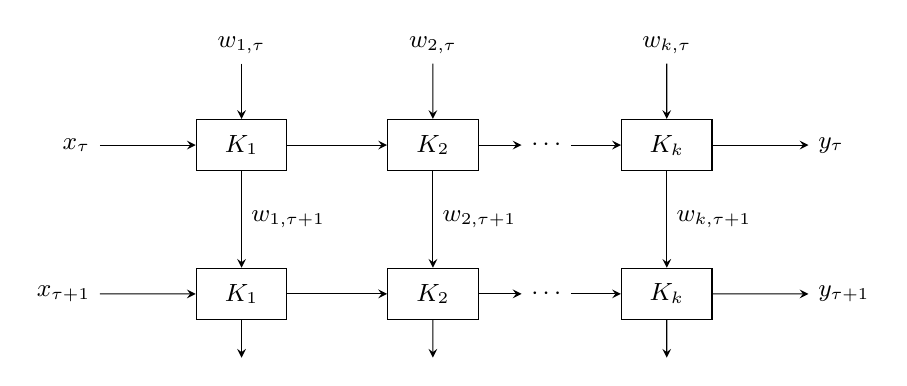
\begin{tikzpicture}[>=stealth,scale=.9,every node/.style={font=\small}]
 \node[draw,minimum width=1.15cm,minimum height=.65cm] (a1) at (0,0) {$K_1$};
 \node[draw,minimum width=1.15cm,minimum height=.65cm] (a2) at (2.7,0) {$K_2$};
 \node (ad) at (4.3,0) {$\cdots$};
 \node[draw,minimum width=1.15cm,minimum height=.65cm] (ak) at (6,0) {$K_k$};
 \node[draw,minimum width=1.15cm,minimum height=.65cm] (b1) at (0,-2.1) {$K_1$};
 \node[draw,minimum width=1.15cm,minimum height=.65cm] (b2) at (2.7,-2.1) {$K_2$};
 \node (bd) at (4.3,-2.1) {$\cdots$};
 \node[draw,minimum width=1.15cm,minimum height=.65cm] (bk) at (6,-2.1) {$K_k$};
 \draw[->] (-2,0) node[left] {$x_\tau$} -- (a1);
 \draw[->] (a1) -- (a2);
 \draw[->] (a2) -- (ad);
 \draw[->] (ad) -- (ak);
 \draw[->] (ak) -- (8,0) node[right] {$y_\tau$};
 \draw[->] (-2,-2.1) node[left] {$x_{\tau+1}$} -- (b1);
 \draw[->] (b1) -- (b2);
 \draw[->] (b2) -- (bd);
 \draw[->] (bd) -- (bk);
 \draw[->] (bk) -- (8,-2.1) node[right] {$y_{\tau+1}$};
 \draw[->] (0,1.15) node[above] {$w_{1,\tau}$} -- (a1.north);
 \draw[->] (2.7,1.15) node[above] {$w_{2,\tau}$} -- (a2.north);
 \draw[->] (6,1.15) node[above] {$w_{k,\tau}$} -- (ak.north);
 \draw[->] (a1.south) -- node[right] {$w_{1,\tau+1}$} (b1.north);
 \draw[->] (a2.south) -- node[right] {$w_{2,\tau+1}$} (b2.north);
 \draw[->] (ak.south) -- node[right] {$w_{k,\tau+1}$} (bk.north);
 \draw[->] (b1.south) -- (0,-3);
 \draw[->] (b2.south) -- (2.7,-3);
 \draw[->] (bk.south) -- (6,-3);
\end{tikzpicture}
\caption{Two ticks of the cascade.  Each $K_j$ represents
$n^{k-1}$ disjoint calls along axis $j$.  Horizontal arrows carry
$N$ data coordinates; the separate vertical arrows carry each
axis's $rn^{k-1}$ persistent state coordinates.}
\label{corner:fig:cascade}
\end{figure}

With data coordinates listed before all state coordinates, the
top-left block of $\mathcal K_{k,t}$ is
\[
 A_{k,t}=\mathcal T_t(H_k),\qquad H_k(z)=H(z)^{\otimes k}.
\]
Indeed the direct series response composes the lifts of $H$ on all
axes.  The top-right block $E_t$ consists of the first $t$ coefficients
of $E(z)=[E_1(z)\ \cdots\ E_k(z)]$, where
\begin{equation}
 E_j(z)=I_n^{\otimes(j-1)}\otimes
        \bigl(C(I_r-zD)^{-1}\bigr)\otimes H(z)^{\otimes(k-j)}.
 \label{corner:eq:state-response}
\end{equation}
An initial state at axis $j$ passes through that axis's state-to-data
map and then through the later axes; the earlier axes do not act on
this contribution.  This proves \cref{corner:eq:state-response} as
well as the direct response, including the order of all factors.

\begin{lemma}[Uniform cascade estimate]
\label{corner:lem:cascade}
For each fixed cell $K$ as in \cref{corner:eq:cell}, there is a constant $C_K$
such that, for every $k,t\ge1$ and $N=n^k$,
\begin{equation}
 p\bigl(\mathcal T_t(H^{\otimes k})\bigr)
 \le tk n^{k-1}p(K)
       +C_K\bigl(Nt\log(2t)+(k+1)^3N\bigr).
 \label{corner:eq:cascade-bound}
\end{equation}
The constant is independent of $t$, $k$, and any scalars used for
coefficient interpolation.
\end{lemma}

\begin{proof}
If $r=0$, the state is absent and $H=M=K$ is constant.  The exact
tensor and direct-sum laws already give the assertion.  Suppose
$r\ge1$ and introduce polynomial matrices and scalar polynomials
\[
 \begin{gathered}
 a(z)=\det(I_r-zD),\qquad R(z)=\operatorname{adj}(I_r-zD),\\
 F(z)=a(z)M+zCR(z)B,\qquad
 b(z)=\det F(z),\qquad J(z)=\operatorname{adj}F(z).
 \end{gathered}
\]
Then $H=F/a$, $H^{-1}=aJ/b$, $a(0)=1$, and
$b(0)=\det M\ne0$.  We have
\[
 \deg a\le r,\quad\deg R\le r-1,\quad
 \deg F\le r,\quad\deg b\le nr,\quad\deg J\le(n-1)r.
\]
For $n=1$ the adjugate $J$ is the constant $1$, as required by
these formulas.  Cancelling the later-axis responses in
\cref{corner:eq:state-response} gives
\[
 H_k^{-1}E_j
 =(H^{-1})^{\otimes(j-1)}\otimes(JCR/b)
                         \otimes I_n^{\otimes(k-j)}.
\]
Thus $q_k=b^k$ clears the entire matrix $H_k^{-1}E$.  Its $j$th
cleared block is the following explicit polynomial map $W_j\to\C^N$:
\begin{equation}
 Q_{k,j}(z)
 =a(z)^{j-1}b(z)^{k-j}\Bigl(
    J(z)^{\otimes(j-1)}\otimes\bigl(J(z)CR(z)\bigr)
                     \otimes I_n^{\otimes(k-j)}\Bigr).
 \label{corner:eq:cleared-state}
\end{equation}
Its degree is at most
\[
 (j-1)r+(k-j)nr+(j-1)(n-1)r+(nr-1)=knr-1.
\]
The scalar $q_k$ has degree at most $knr$ and has nonzero constant
term.  The identities also hold when any of the displayed matrix
polynomials vanish.

Here is an explicit DAG bound for the nonzero time coordinates of
$Q_k(z)w=\sum_{j=1}^kQ_{k,j}(z)w_j$.  Put $m=knr$, and choose $m$
distinct complex evaluation points.  Because
\cref{corner:eq:cleared-state} is polynomial, no avoidance of poles
is needed.  At one evaluation point, a rectangular application of
$JCR$ on its $r$-axis costs at most $2rN$ scalar gates.  Applying
$J$ on the preceding $j-1$ axes costs at most $2n(j-1)N$ gates,
by doing the fixed $n\times n$ map on all fibers of each axis.
The scalar factor costs at most $N$ gates.  Adding the $k$
contributions costs at most $(k-1)N$ more.  One evaluation therefore
uses at most
\[
 \bigl(nk(k-1)+2(r+1)k-1\bigr)N=O_K(k^2N)
\]
gates.  All local entries and scalar powers here are prechosen
constants.  Applying the inverse scalar Vandermonde matrix to the
$m$ evaluations, separately on each of the $N$ coordinates, recovers
all $m$ coefficient vectors using at most $2m^2N$ further scalar
gates.  The total is $O_K((k+1)^3N)$.
For any run length $t$, keep only the first $\min(t,m)$ coefficient
vectors; all other rows of the truncated response are zero.  This
bound is consequently uniform in $t$.

Set $P=\mathcal T_t(1/q_k)$ and
$A'=A_{k,t}(P\otimes I_N)$.  In formal series modulo $z^t$,
$A'^{-1}E_t$ is precisely the coefficient map of
$q_kH_k^{-1}E=Q_k$ just constructed.  Hence
\cref{lem:shear-dag}, with zero output rows omitted, bounds the
price of the shear with block $-A'^{-1}E_t$ by
$O_K((k+1)^3N)$.  This uses only the rectangular shear law, not a
price bound for an arbitrary invertible circuit output.

Now form the exact product
\begin{equation}
 \mathcal K_{k,t}
 \begin{pmatrix}P\otimes I_N&0\\0&I\end{pmatrix}
 \begin{pmatrix}I&-A'^{-1}E_t\\0&I\end{pmatrix}.
 \label{corner:eq:state-elimination}
\end{equation}
Its top row of blocks is $(A',0)$.  Each factor is invertible, and
$A'$ is invertible because $H(0)=M$ and $q_k(0)\ne0$.  Therefore
the other diagonal block of this lower triangular product is also
invertible.  By \cref{lem:triangular} its price is at least $p(A')$.
There are $tkn^{k-1}$ cell calls in $\mathcal K_{k,t}$, so
\[
 p(A')\le tkn^{k-1}p(K)+N p(P)+O_K((k+1)^3N).
\]
Here the tensor and direct-sum laws price the scalar preprocessing
by $Np(P)$, including its identity on the state.  Finally
$A_{k,t}=A'(P^{-1}\otimes I_N)$ and inverse symmetry give
\[
 p(A_{k,t})\le tkn^{k-1}p(K)+2Np(P)+O_K((k+1)^3N).
\]
Apply \cref{lem:scalar-convolution} to $P$.  Its bound is uniform
even though $q_k$ varies with $k$, proving
\cref{corner:eq:cascade-bound}.
\end{proof}

\subsection{Proof of the corner law and its circuit consequence}

\begin{proof}[Proof of \cref{thm:corner}]
Independent row and column permutations move $M$ to the top-left
corner and preserve $p(K)$.  Write the resulting matrix as in
\cref{corner:eq:cell}.  If the complementary width is zero the claim
is equality; otherwise apply \cref{corner:lem:cascade}.  The matrix
$A_{k,t}=\mathcal T_t(H^{\otimes k})$ is lower triangular in time
with $t$ identical diagonal blocks $M^{\otimes k}$.  Thus
\cref{lem:triangular} and the tensor law imply
\[
 p(A_{k,t})\ge t p(M^{\otimes k})
             =tkn^{k-1}p(M).
\]
Fix $K,n,r$ first and use the bound of
\cref{corner:eq:cascade-bound}.  For example, choose
$t=t(k)=2^{\lceil8\log_2(k+1)\rceil}$, so
$(k+1)^8\le t<2(k+1)^8$.  Division by $tkn^{k-1}=tkN/n$ gives
\[
 p(M)\le p(K)+C_K n\left(
       \frac{\log(2t)}{k}+\frac{(k+1)^3}{tk}\right).
\]
Both errors tend to zero.  The matrices $M$ and $K$ in this real
inequality are fixed, so it proves the exact inequality
$p(M)\le p(K)$.  No continuity assertion about the price, or
limiting circuit for a matrix, has been used.  A zero-size submatrix,
if allowed, can simply be omitted and assigned price zero.
\end{proof}

\begin{corollary}[A universal one-way DAG price bound]
\label{cor:dag-price}
If $G\in\GL_m(\C)$ has a permitted linear DAG with $l$ scalar
gates, then
\[
 p(G)\le s(G)\le 8l+2m.
\]
The bound holds with the same constants for all dimensions and all
matrix families, without requiring a DAG for $G^{-1}$.
\end{corollary}

\begin{proof}
$G$ is an invertible square submatrix of
$\begin{pmatrix}I_m&G\\0&I_m\end{pmatrix}$, so
\cref{thm:corner} gives its first inequality, and
\cref{lem:shear-dag} gives the second.  Although the proof of the
corner law fixed each individual matrix while taking a limit, the
resulting inequality is exact for every finite matrix.  The numerical
constants here come entirely from the dirty scratch simulation.
\end{proof}
